\let\negmedspace\undefined
\let\negthickspace\undefined
\documentclass[journal]{IEEEtran}
\usepackage[a5paper, margin=10mm, onecolumn]{geometry}
%\usepackage{lmodern} % Ensure lmodern is loaded for pdflatex
\usepackage{tfrupee} % Include tfrupee package

\setlength{\headheight}{1cm} % Set the height of the header box
\setlength{\headsep}{0mm}     % Set the distance between the header box and the top of the text

\usepackage{gvv-book}
\usepackage{gvv}
\usepackage{cite}
\usepackage{amsmath,amssymb,amsfonts,amsthm}
\usepackage{algorithmic}
\usepackage{graphicx}
\usepackage{textcomp}
\usepackage{xcolor}
\usepackage{txfonts}
\usepackage{listings}
\usepackage{enumitem}
\usepackage{mathtools}
\usepackage{gensymb}
\usepackage{comment}
\usepackage[breaklinks=true]{hyperref}
\usepackage{tkz-euclide} 
\usepackage{listings}
% \usepackage{gvv}                                        
\def\inputGnumericTable{}                                 
\usepackage[latin1]{inputenc}                                
\usepackage{color}                                            
\usepackage{array}                                            
\usepackage{longtable}                                       
\usepackage{calc}                                             
\usepackage{multirow}                                         
\usepackage{hhline}                                           
\usepackage{ifthen}                                           
\usepackage{lscape}
\begin{document}

\bibliographystyle{IEEEtran}
\vspace{3cm}

\title{5.8.31}
\author{EE25BTECH11033 - Kavin}
% \maketitle
% \newpage
% \bigskip
{\let\newpage\relax\maketitle}

\renewcommand{\thefigure}{\theenumi}
\renewcommand{\thetable}{\theenumi}
\setlength{\intextsep}{10pt} % Space between text and floats
\textbf{Question}:\\
In a $\triangle ABC,  \angle C=3 \angle B=2(\angle A+\angle B)$.  Find the three angles. 
\bigskip

\textbf{Solution}:\\
In a $\triangle ABC$ , the sum of interior angles is equal to $180$.
\begin{align}
    \angle A + \angle B + \angle C = 180
\end{align}
Also,
\begin{align}
    \angle C - 3\angle B = 0
\end{align}
\begin{align}
    2\angle A - \angle B = 0
\end{align}
On putting the above equations in a matrix we will get,
\begin{align}
    \myvec{ 1 & 1 & 1\\0 & -3 & 1\\2 & -1 & 0}\myvec{\angle A \\ \angle B \\ \angle C} = \myvec{180\\0\\0}
\end{align}
The augmented matrix is given by,
\begin{align}
    \augvec{3}{1}{1 & 1 & 1 & 180\\0 & -3 & 1 & 0\\2 & -1 & 0 & 0}
\end{align}
\begin{align}
    R_3 \to R_3 - 2R_1 \implies \augvec{3}{1}{1 & 1 & 1 & 180 \\ 0 & -3 & 1 & 0 \\ 0 & -3 & -2 & -360}
\end{align}
\begin{align}
    R_2 \to -1/3 R_2  \implies \augvec{3}{1}{1 & 1 & 1 & 180 \\ 0 & 1 & -1/3 & 0 \\ 0 & -3 & -2 & -360}
\end{align}
\begin{align}
    R_1 \to R_1 - R_2\ \text{and}\ R_3 \to R_3 + 3R_2 \implies \augvec{3}{1}{1 & 0 & 4/3 & 180 \\ 0 & 1 & -1/3 & 0 \\ 0 & 0 & -3 & -360}
\end{align}
\begin{align}
    R_3 \to -1/3 R_3 \implies \augvec{3}{1}{1 & 0 & 4/3 & 180 \\ 0 & 1 & -1/3 & 0 \\ 0 & 0 & 1 & 120}
\end{align}
\begin{align}
    R_1 \to R_1 - 4/3 R_3\ \text{and}\ R_2 \to R_2 + 1/3 R_3\implies \augvec{3}{1}{1 & 0 & 0 & 20 \\ 0 & 1 & 0 & 40 \\ 0 & 0 & 1 & 120}
\end{align}\\
\bigskip

\begin{align}
    \implies \myvec{\angle A \\ \angle B \\ \angle C} = \myvec{20\\40\\120}
\end{align}
Therefore,
\begin{align*}
\angle A = 20\degree \ \ \ \ \ 
\angle B = 40\degree
\end{align*}
\begin{align*}
\angle C = 120\degree
\end{align*}

\begin{figure}[H]
\begin{center}
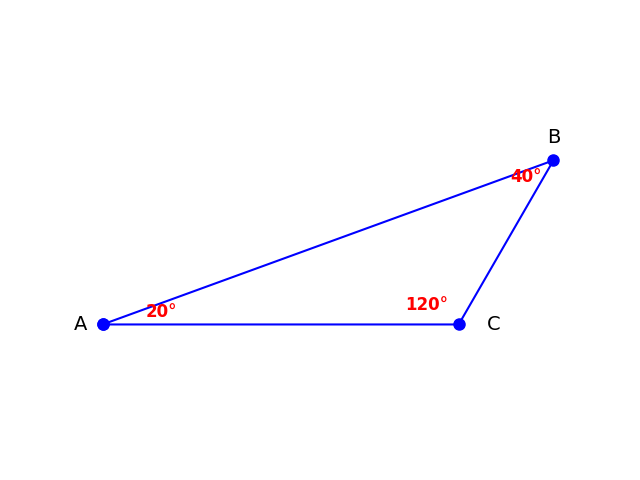
\includegraphics[width=0.7\columnwidth]{figs/fig.png}
\end{center}
\label{fig:Fig1}
\end{figure}
\end{document}


